\documentclass[border=2pt]{standalone}
\usepackage{tikz}
\usepackage{amsmath,amssymb}
\begin{document}
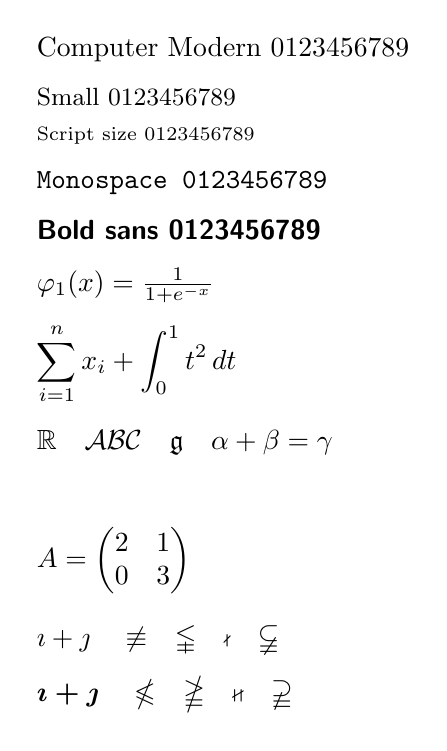
\begin{tikzpicture}
  \node[anchor=west] at (0,0) {Computer Modern 0123456789};
  \node[anchor=west,font=\small] at (0,-.6) {Small 0123456789};
  \node[anchor=west,font=\scriptsize] at (0,-1.1) {Script size 0123456789};
  \node[anchor=west,font=\ttfamily] at (0,-1.7) {Monospace 0123456789};
  \node[anchor=west,font=\sffamily\bfseries] at (0,-2.3) {Bold sans 0123456789};
  \node[anchor=west] at (0,-3) {$\varphi_1(x)=\frac{1}{1+e^{-x}}$};
  \node[anchor=west] at (0,-4) {$\displaystyle\sum_{i=1}^{n} x_i+\int_0^1 t^2\,dt$};
  \node[anchor=west] at (0,-5) {$\mathbb{R}\quad\mathcal{ABC}\quad\mathfrak{g}\quad\alpha+\beta=\gamma$};
  \node[anchor=west] at (0,-6.5) {$A=\begin{pmatrix}2&1\\0&3\end{pmatrix}$};
  \node[anchor=west] at (0,-7.5) {$\imath+\jmath\quad\not\equiv\quad\lvertneqq\quad\nshortmid\quad\varsubsetneqq$};
  \node[anchor=west] at (0,-8.2) {$\boldsymbol{\imath+\jmath}\quad\nleqslant\quad\ngeqq\quad\nshortparallel\quad\varsupsetneqq$};
\end{tikzpicture}
\end{document}
